\documentclass{report}
\usepackage{graphicx}
\usepackage{hyperref}
\usepackage[utf8]{inputenc}
\usepackage[T1]{fontenc}
\usepackage{float}

\title{Creación de una Interfaz Gráfica para Cargar y Visualizar Imágenes JPEG}
\author{Angel Miranda San Martín}
\date{5 de Octubre de 2024}

\begin{document}

  \begin{titlepage}
    \begin{minipage}{0.5\textwidth}
      \flushleft
      \includegraphics[width=2cm]{image/logo-ipn-guinda}
    \end{minipage}
    \begin{minipage}{0.5\textwidth}
      \flushright
      \includegraphics[width=3cm]{image/logo-escom}
    \end{minipage}
    \vspace{1cm}
    \begin{center}
      \Huge \textbf{ Creación de una Interfaz Gráfica para Cargar y Visualizar Imágenes JPEG}
      \vspace{1cm}

      \Large Grupo: 4BV1
      \vspace{1cm}

      Profesor: De la O Torres Saúl
      \vspace{1cm}

      Alumno: Miranda San Martin Angel
      \vspace{0.5cm}

      Boleta: 2023630959
      \vspace{2cm}

      \large Instituto Politécnico Nacional / Escuela Superior de Cómputo
      \vspace{1cm}

      \large Fecha de entrega: 07/10/2024
    \end{center}
  \end{titlepage}

  \tableofcontents


  \chapter{Introducción}\label{ch:introduccion}
  El procesamiento digital de imágenes es un campo interdisciplinario que involucra conceptos de matemáticas, informática, y electrónica, y su aplicación se extiende a una gran variedad de áreas como la medicina, la astronomía, el reconocimiento de patrones, la visión por computadora, y más.
  Su objetivo principal es la manipulación de imágenes digitales a través de algoritmos, permitiendo desde la corrección de color y brillo hasta la detección de características avanzadas.

  En esta práctica, el enfoque fue desarrollar una aplicación en Java que permita cargar, visualizar y aplicar transformaciones básicas a imágenes en formato JPEG. Para ello, se emplearon las APIs de \textbf{Swing} y \textbf{AWT} (Abstract Window Toolkit), que proporcionan un conjunto de componentes gráficos y herramientas que facilitan la creación de interfaces gráficas de usuario (GUI).

  \textbf{Swing} es una extensión de AWT que ofrece un conjunto más amplio de componentes GUI (botones, tablas, listas, etc.) y permite mayor personalización.
  AWT, por otro lado, proporciona los componentes gráficos básicos y permite manipular gráficos directamente a través de objetos como \texttt{BufferedImage}, fundamental para el procesamiento de imágenes en Java.

  Para comprender mejor esta práctica, es crucial tener conocimientos previos sobre:
  \begin{itemize}
    \item \textbf{Modelos de color}: Las imágenes digitales suelen representarse mediante el modelo RGB (Rojo, Verde, Azul), donde cada píxel tiene valores que representan la intensidad de cada color.
    \item \textbf{Manipulación de píxeles}: Procesar una imagen implica modificar sus píxeles uno por uno, lo que puede hacerse para ajustar brillo, contraste, aplicar filtros, entre otros.
    \item \textbf{Interfaces gráficas en Java}: Comprender cómo funciona la arquitectura de Swing y AWT facilita la creación de aplicaciones interactivas y con componentes visuales.
  \end{itemize}


  \chapter{Desarrollo}\label{ch:desarrollo}


  \section{Estructura del Proyecto}\label{sec:estructura-del-proyecto}
  El proyecto está dividido en varias clases, que se encargan de tareas específicas para modularizar el código y facilitar su mantenimiento.
  La estructura sigue un diseño orientado a objetos, donde cada clase tiene una responsabilidad claramente definida.
  Las principales clases son:

  \subsection{Bootstrap.java}\label{subsec:bootstrap.java}
  La clase \texttt{Bootstrap} actúa como el punto de entrada de la aplicación.
  En su método principal, utiliza el patrón de diseño \textbf{Singleton} para crear instancias de los procesadores de píxeles y de la interfaz gráfica principal (\texttt{MainFrame}). Este patrón asegura que solo exista una instancia de cada componente, lo que optimiza el uso de recursos y simplifica la gestión de dependencias.

  La clase crea un objeto de \texttt{BufferedImageContainer}, que es el contenedor de la imagen cargada, y un \texttt{ImageProcessor}, que coordina el procesamiento de la imagen a través de los distintos filtros y ajustes.

  \subsection{ImageProcessor.java}\label{subsec:imageprocessor.java}
  El \texttt{ImageProcessor} es el encargado de gestionar el ciclo de procesamiento de la imagen.
  Recibe una lista de procesadores de píxeles (\texttt{PixelProcessor}) que se aplican secuencialmente a cada píxel de la imagen.
  Este patrón modular permite añadir fácilmente nuevos filtros en el futuro sin afectar la arquitectura existente.

  Por ejemplo, el procesamiento se realiza recorriendo cada píxel de la imagen, extrayendo sus valores RGB y pasando estos valores por cada uno de los procesadores, como el de brillo o el de contraste.

  \subsection{PixelProcessor.java}\label{subsec:pixelprocessor.java}
  \texttt{PixelProcessor} es una interfaz que define el comportamiento de los procesadores de píxeles.
  Todos los procesadores (brillo, contraste, escala de grises, etc.) implementan esta interfaz, lo que permite intercambiarlos o agregarlos de manera flexible sin modificar el código base del \texttt{ImageProcessor}.

  Cada procesador recibe un \texttt{PixelProcessorContext}, que contiene el valor del píxel actual, su posición (x, y), y la configuración actual (brillo, contraste, etc.). Luego, realiza la transformación correspondiente y devuelve el valor modificado del píxel.

  \subsection{BrightnessPixelProcessor.java}\label{subsec:brightnesspixelprocessor.java}
  Este procesador ajusta el brillo de cada píxel sumando o restando un valor a los canales RGB. Se asegura de que el valor final de cada canal esté en el rango válido de 0 a 255, utilizando las funciones \texttt{Math.min()} y \texttt{Math.max()} para evitar valores fuera del rango.

  \subsection{GrayScalePixelProcessor.java}\label{subsec:grayscalepixelprocessor.java}
  El procesador de escala de grises convierte una imagen en color en una imagen en blanco y negro utilizando una fórmula estándar para combinar los valores RGB en un solo valor de luminosidad.
  Esta fórmula toma un porcentaje de cada canal (30\% de rojo, 59\% de verde y 11\% de azul) para calcular el valor de gris resultante.

  \subsection{BufferedImageContainer.java}\label{subsec:bufferedimagecontainer.java}
  El \texttt{BufferedImageContainer} se encarga de gestionar la imagen cargada y su versión modificada.
  Permite al usuario restaurar la imagen original si es necesario.
  Además, la clase utiliza \texttt{BufferedImageHelper} para crear copias de la imagen original y preservar los datos originales.

  \subsection{MainFrame.java}\label{subsec:mainframe.java}
  La clase \texttt{MainFrame} contiene la ventana principal de la aplicación, que incluye componentes como el \texttt{ControlPanel} y el \texttt{ImagePanel}.
  El \texttt{ControlPanel} permite al usuario ajustar el brillo y el contraste de la imagen, mientras que el \texttt{ImagePanel} muestra la imagen cargada y actualizada en tiempo real.


  \section{Interfaz Gráfica}\label{sec:interfaz-grafica}
  La interfaz gráfica se basa en los componentes de Swing y AWT. A continuación, se describen algunos de los elementos más importantes:

  \subsection{ControlPanel.java}\label{subsec:controlpanel.java}
  El \texttt{ControlPanel} contiene los controles deslizantes (sliders) que permiten al usuario modificar el brillo y el contraste de la imagen cargada.
  Cada cambio en el valor del slider dispara un evento que llama al \texttt{ImageProcessor} para actualizar la imagen en tiempo real.

  \subsection{MenuBar.java}\label{subsec:menubar.java}
  El menú de la aplicación proporciona opciones para cargar y guardar imágenes.
  La opción de cargar permite al usuario seleccionar una imagen JPEG desde su sistema de archivos, mientras que la opción de guardar almacena la imagen modificada en el disco.


  \section{Procesamiento de Imágenes}\label{sec:procesamiento-de-imagenes}
  El procesamiento de imágenes digitales implica la manipulación de los valores de píxeles que componen la imagen.
  En este proyecto, el procesamiento se realiza a nivel de píxel, utilizando los valores RGB para aplicar ajustes de brillo, contraste y convertir a escala de grises.

  Cada píxel es un conjunto de valores que representan la intensidad de los colores primarios (rojo, verde y azul).
  Al modificar estos valores, podemos cambiar la apariencia de la imagen de manera significativa.
  El reto en esta práctica fue manipular estos valores de forma precisa para obtener los resultados deseados.


  \chapter{Funcionamiento}\label{ch:funcionamiento}


  \section{Pantalla Principal}\label{sec:pantalla-principal}
  La pantalla principal de la aplicación muestra un área donde el usuario puede cargar una imagen arrastrando un archivo o haciendo clic para seleccionar una imagen desde el explorador de archivos.

  \begin{figure}[H]
    \centering
    \includegraphics[width=\textwidth]{image/functionality/pantalla-principal}
    \caption{Pantalla principal de la aplicación}\label{fig:pantalla-principal}
  \end{figure}


  \section{Visualización de Imagen}\label{sec:visualizacion-de-imagen}
  Una vez que la imagen es cargada, se puede visualizar dentro del área principal de la aplicación.
  En este caso, la imagen seleccionada es ``La Noche Estrellada`` de Van Gogh.

  \begin{figure}[H]
    \centering
    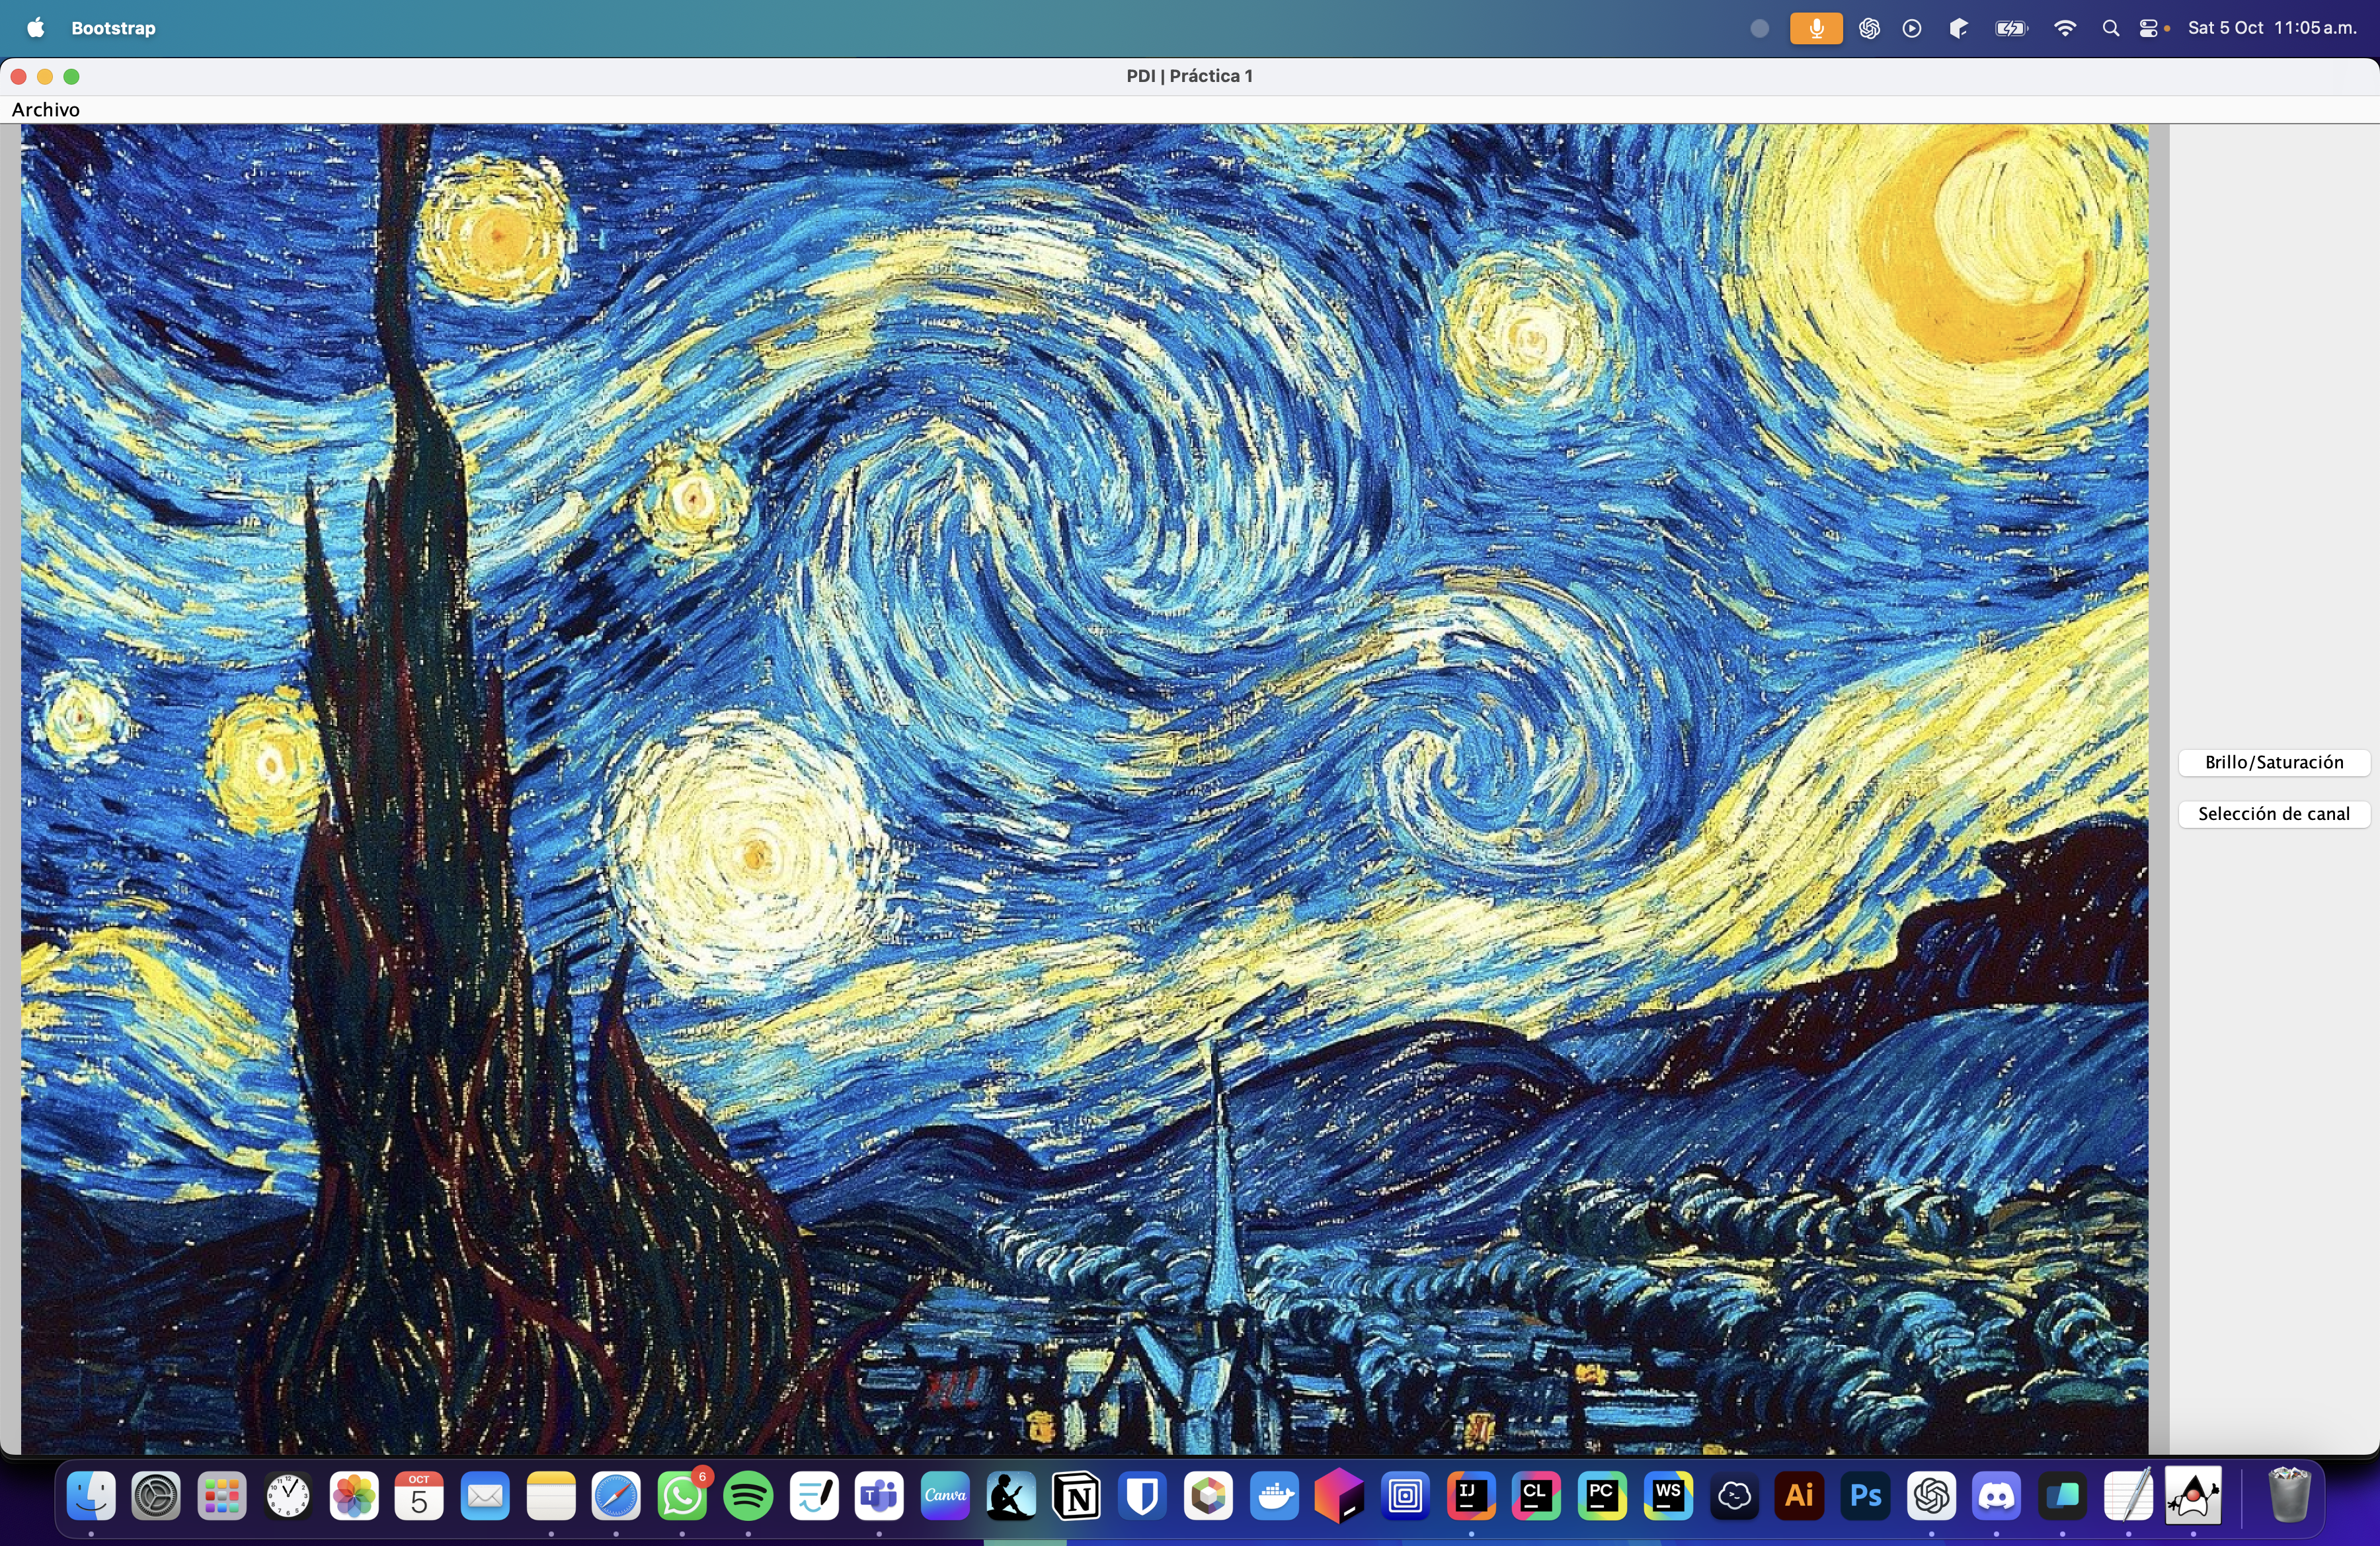
\includegraphics[width=\textwidth]{image/functionality/imagen-cargada}
    \caption{Imagen cargada y visualizada}\label{fig:imagen-cargada}
  \end{figure}


  \section{Ajuste de Brillo y Contraste}\label{sec:ajuste-de-brillo-y-contraste}
  El panel de Brillo y Contraste permite ajustar estos parámetros en tiempo real, mostrando los cambios directamente en la imagen visualizada.

  \begin{figure}[H]
    \centering
    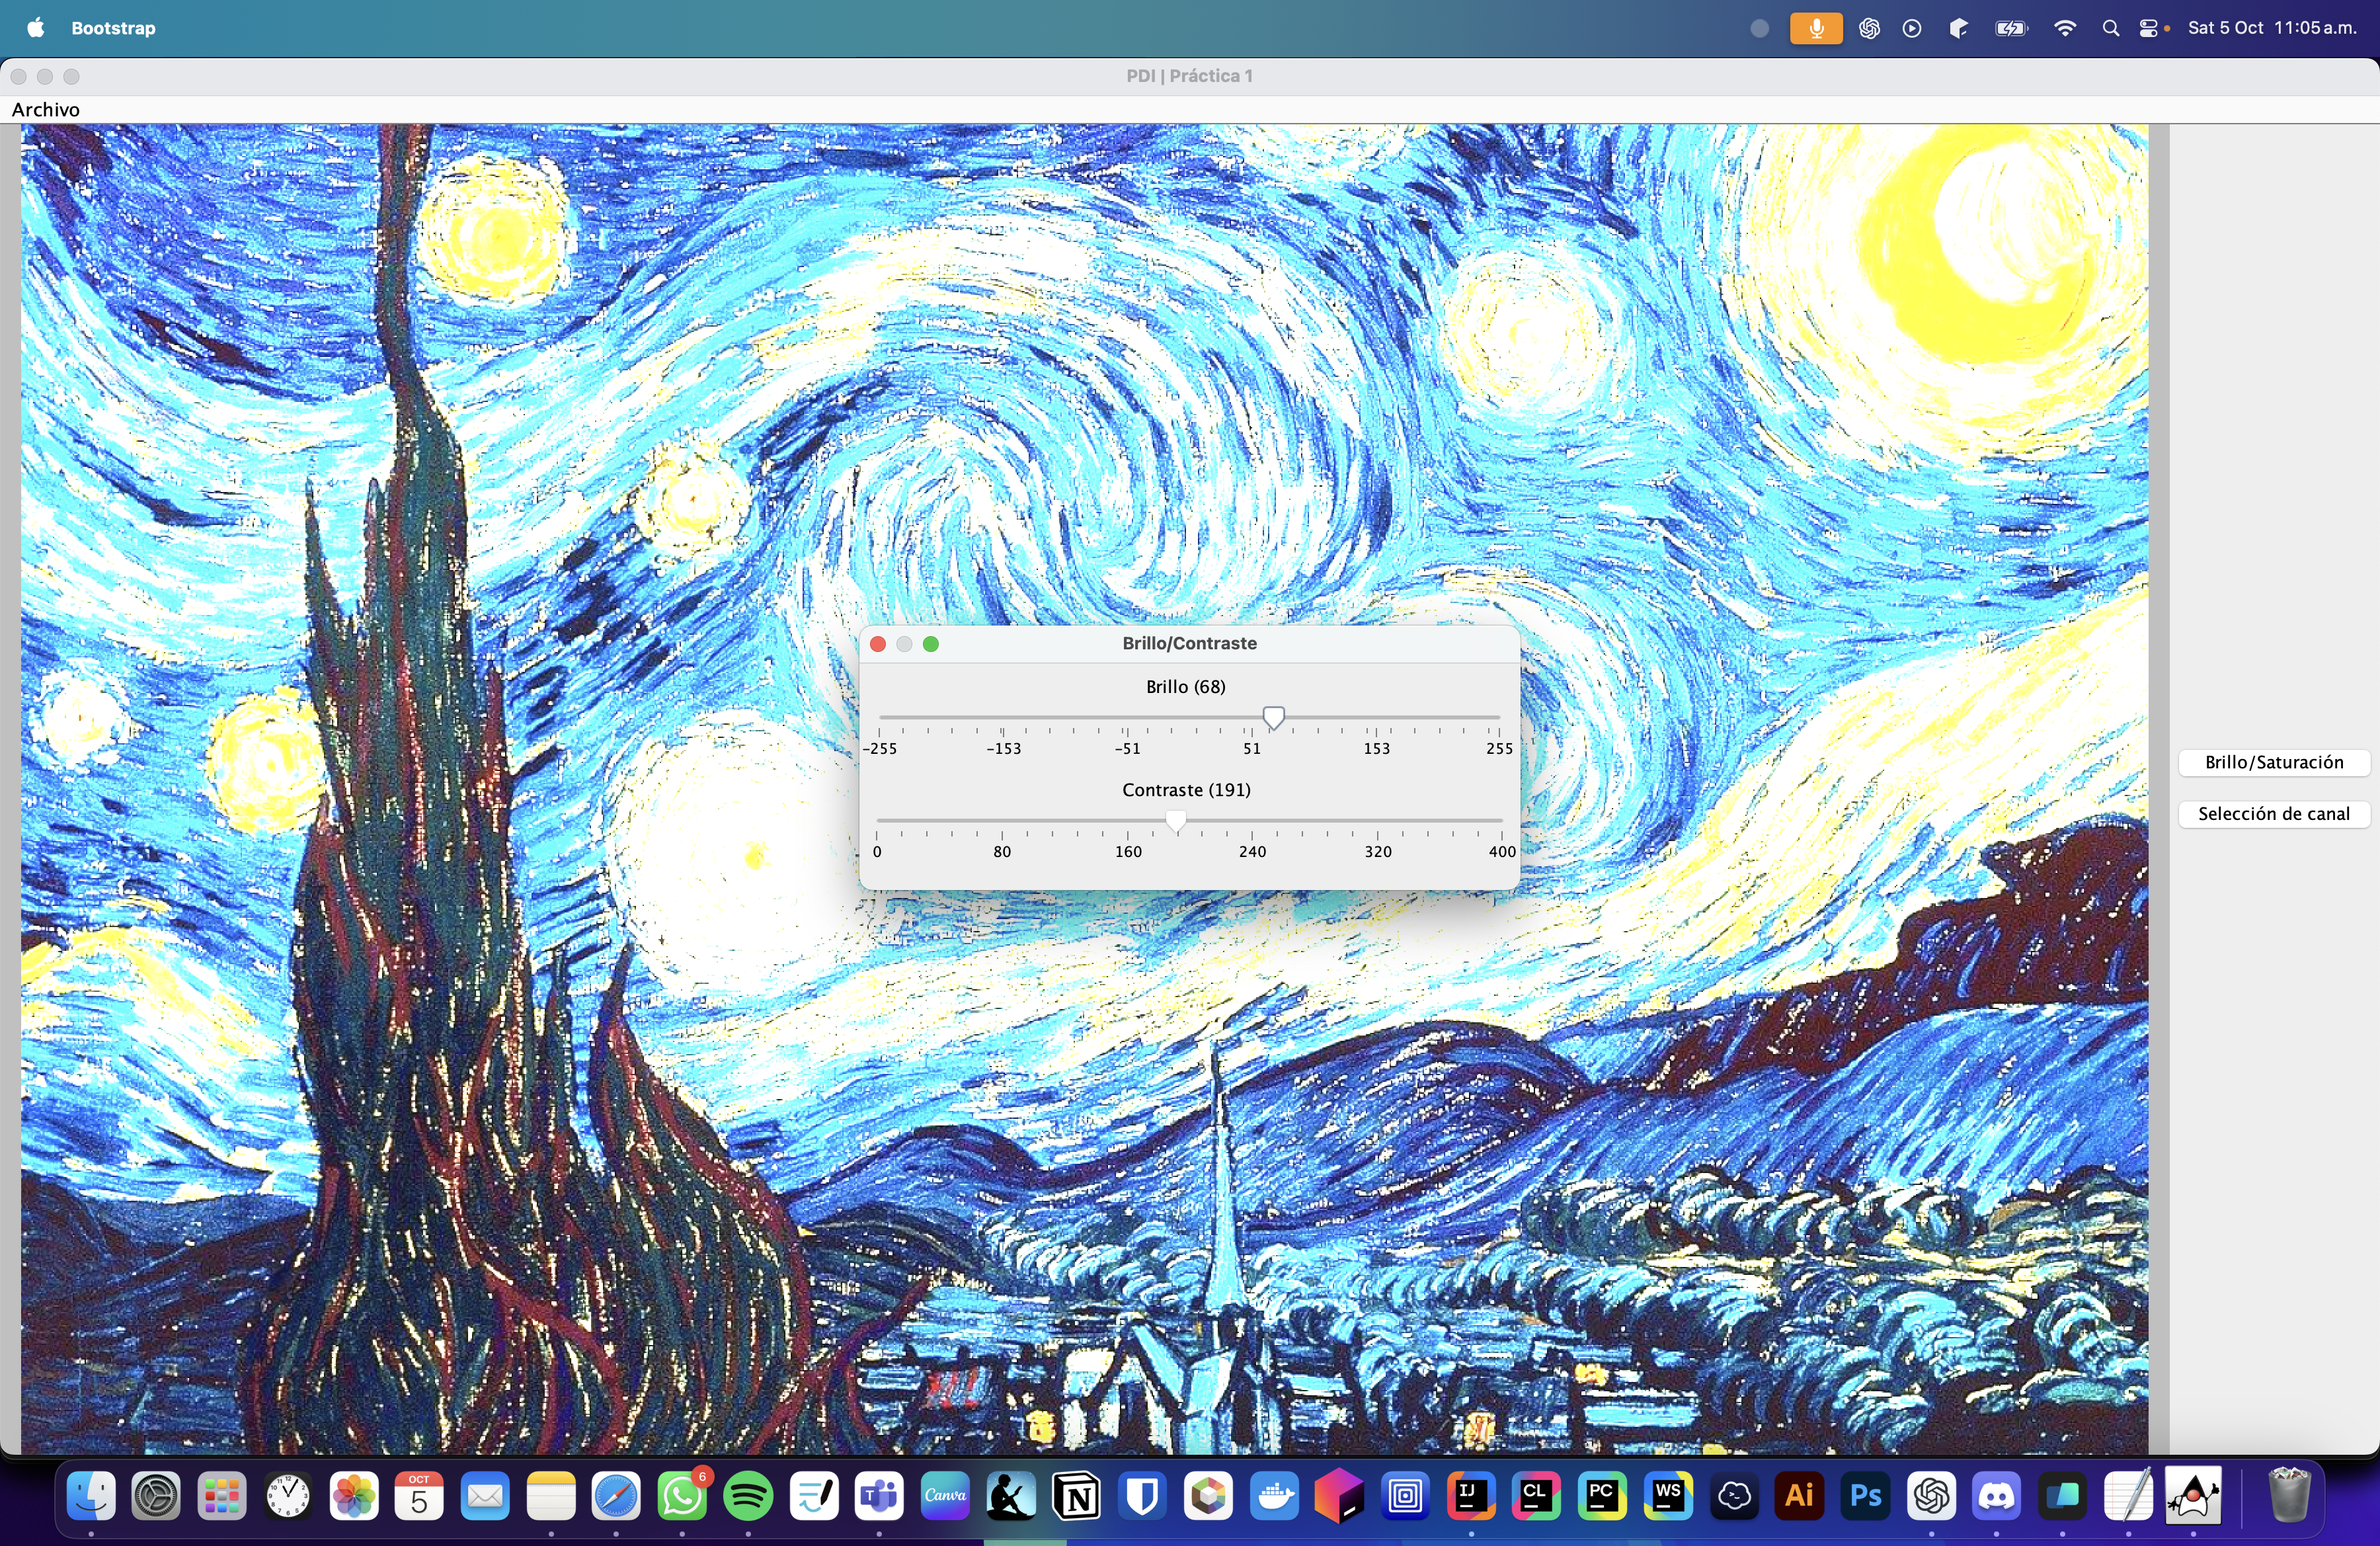
\includegraphics[width=\textwidth]{image/functionality/brillo-contraste}
    \caption{Ajuste de brillo y contraste}\label{fig:brillo-contraste}
  \end{figure}


  \section{Selección de Canal de Color}\label{sec:seleccion-de-canal-de-color}
  El usuario puede seleccionar uno de los canales de color (Rojo, Verde o Azul) para visualizar sólo ese canal de la imagen.

  \subsection{Canal Rojo}\label{subsec:canal-rojo}
  \begin{figure}[H]
    \centering
    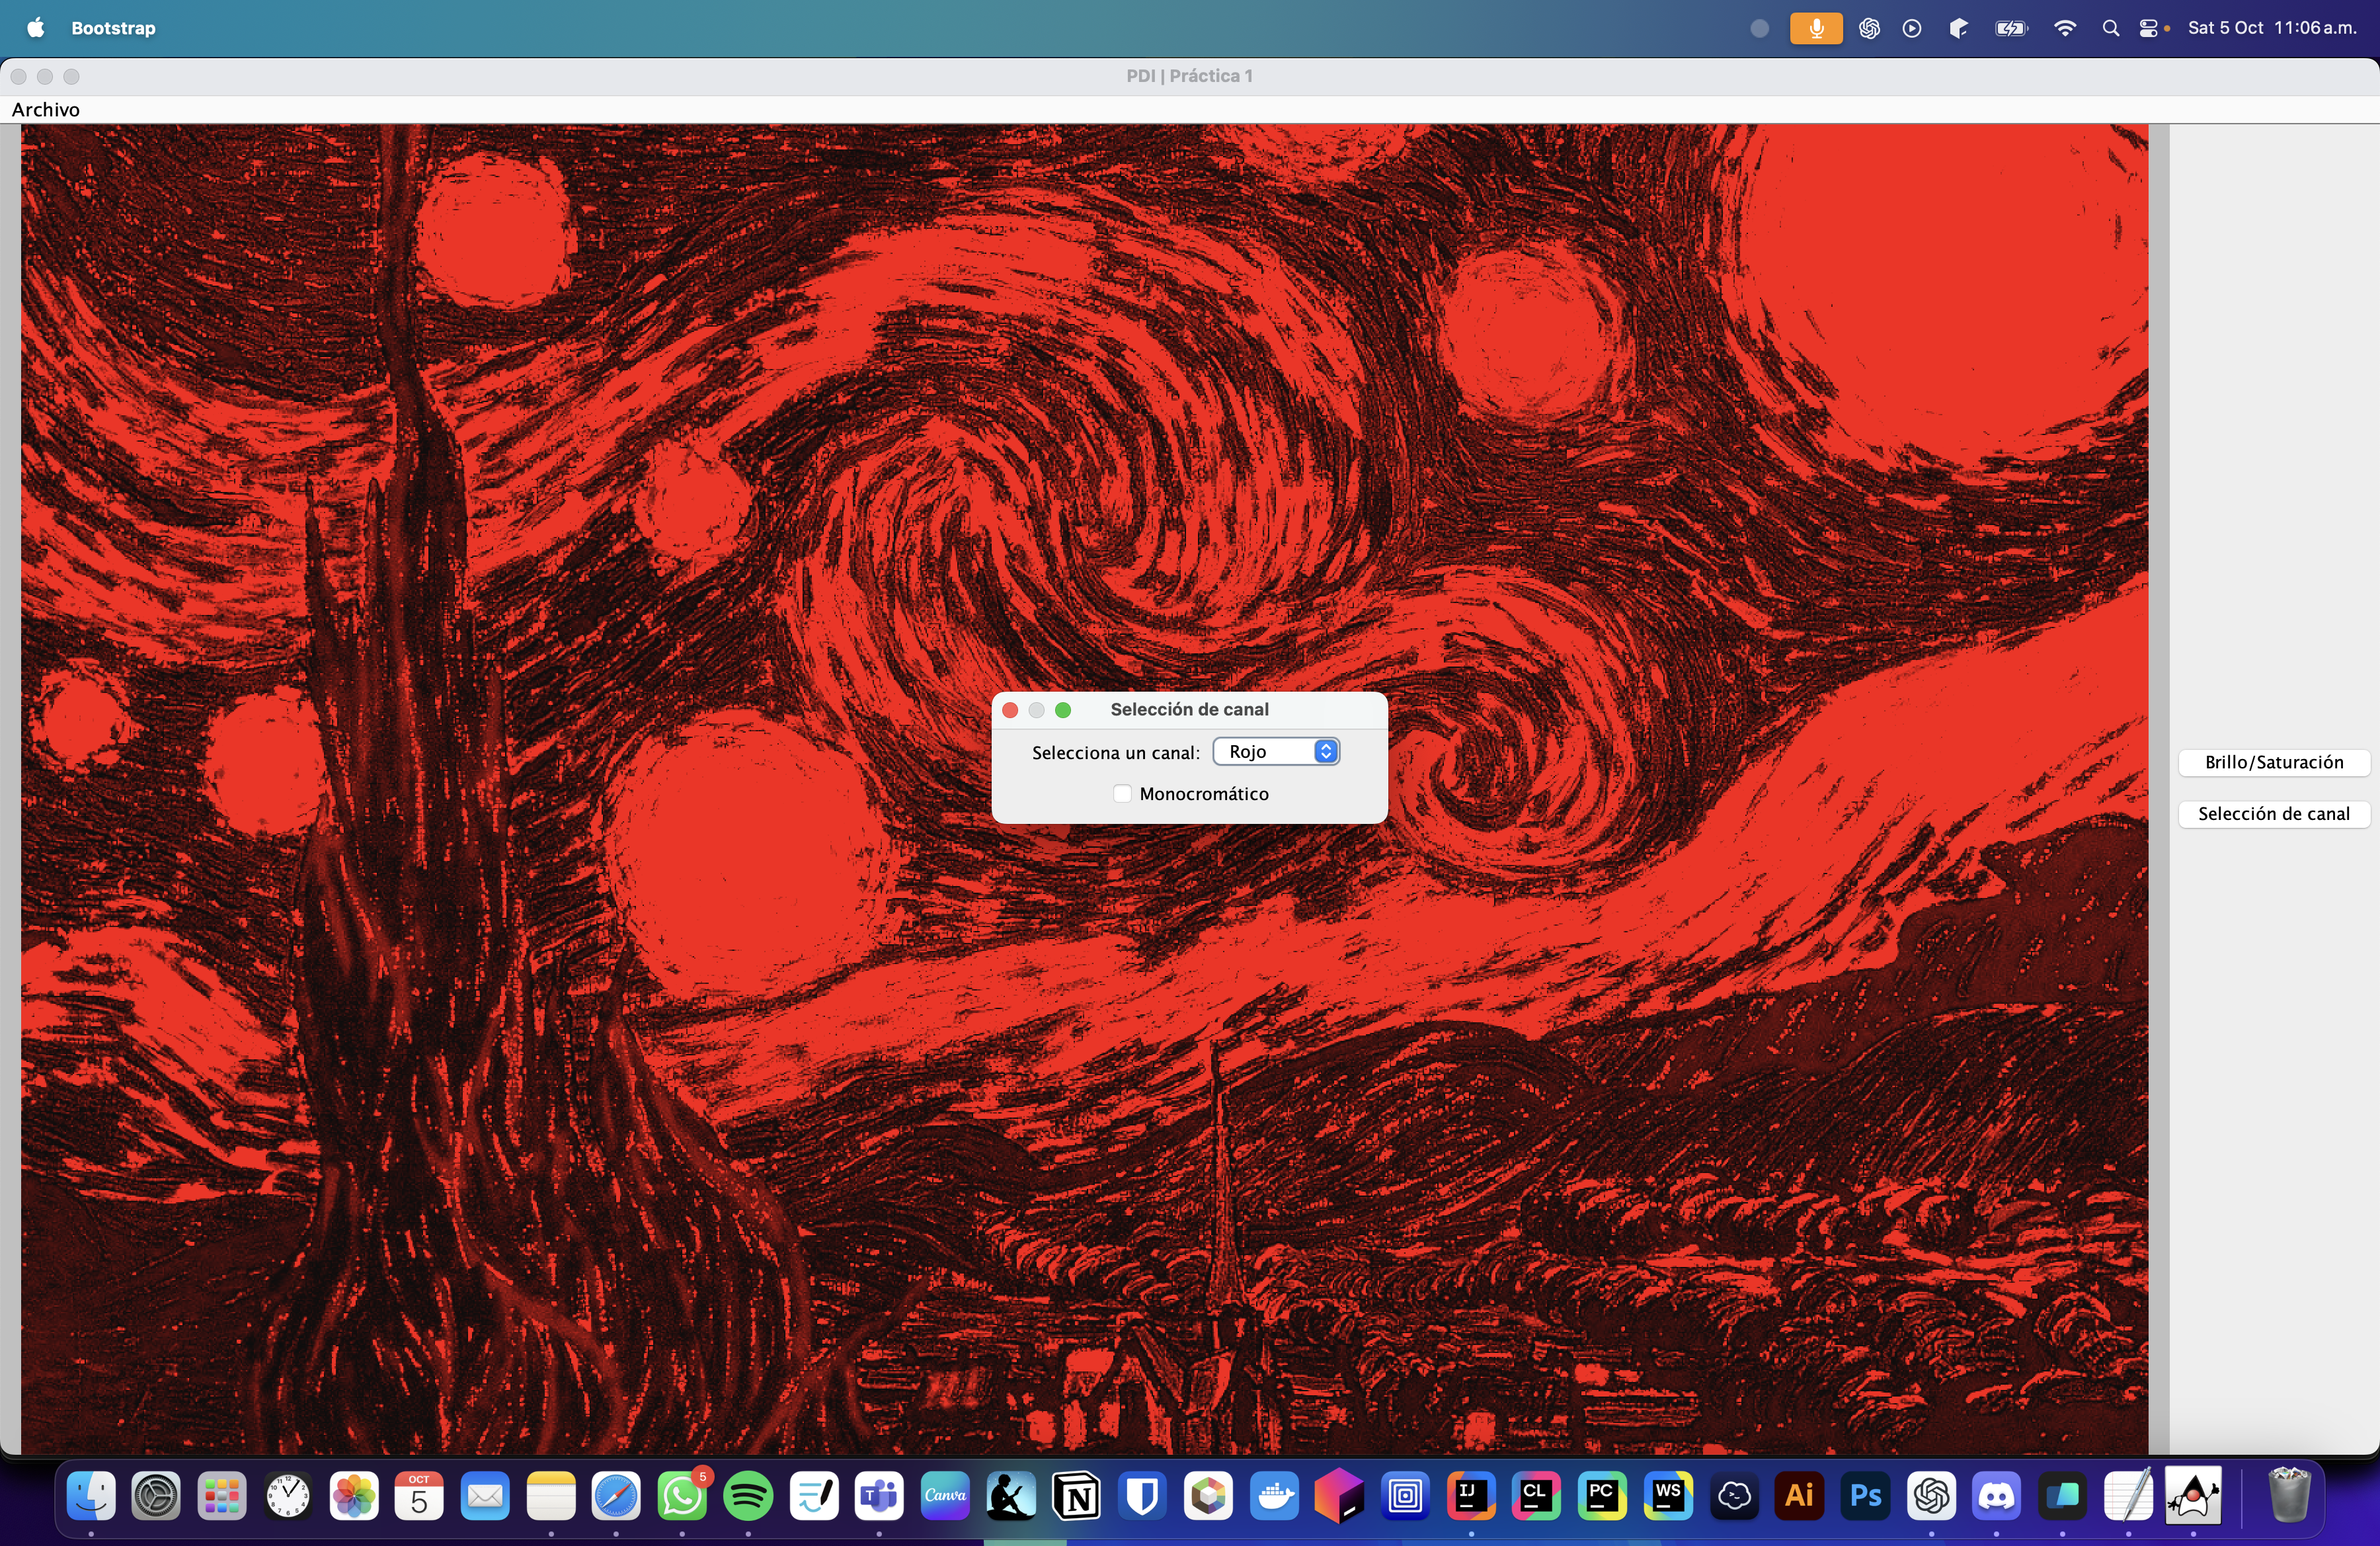
\includegraphics[width=\textwidth]{image/functionality/canal-rojo}
    \caption{Visualización del canal rojo}\label{fig:canal-rojo}
  \end{figure}

  \subsection{Canal Verde}\label{subsec:canal-verde}
  \begin{figure}[H]
    \centering
    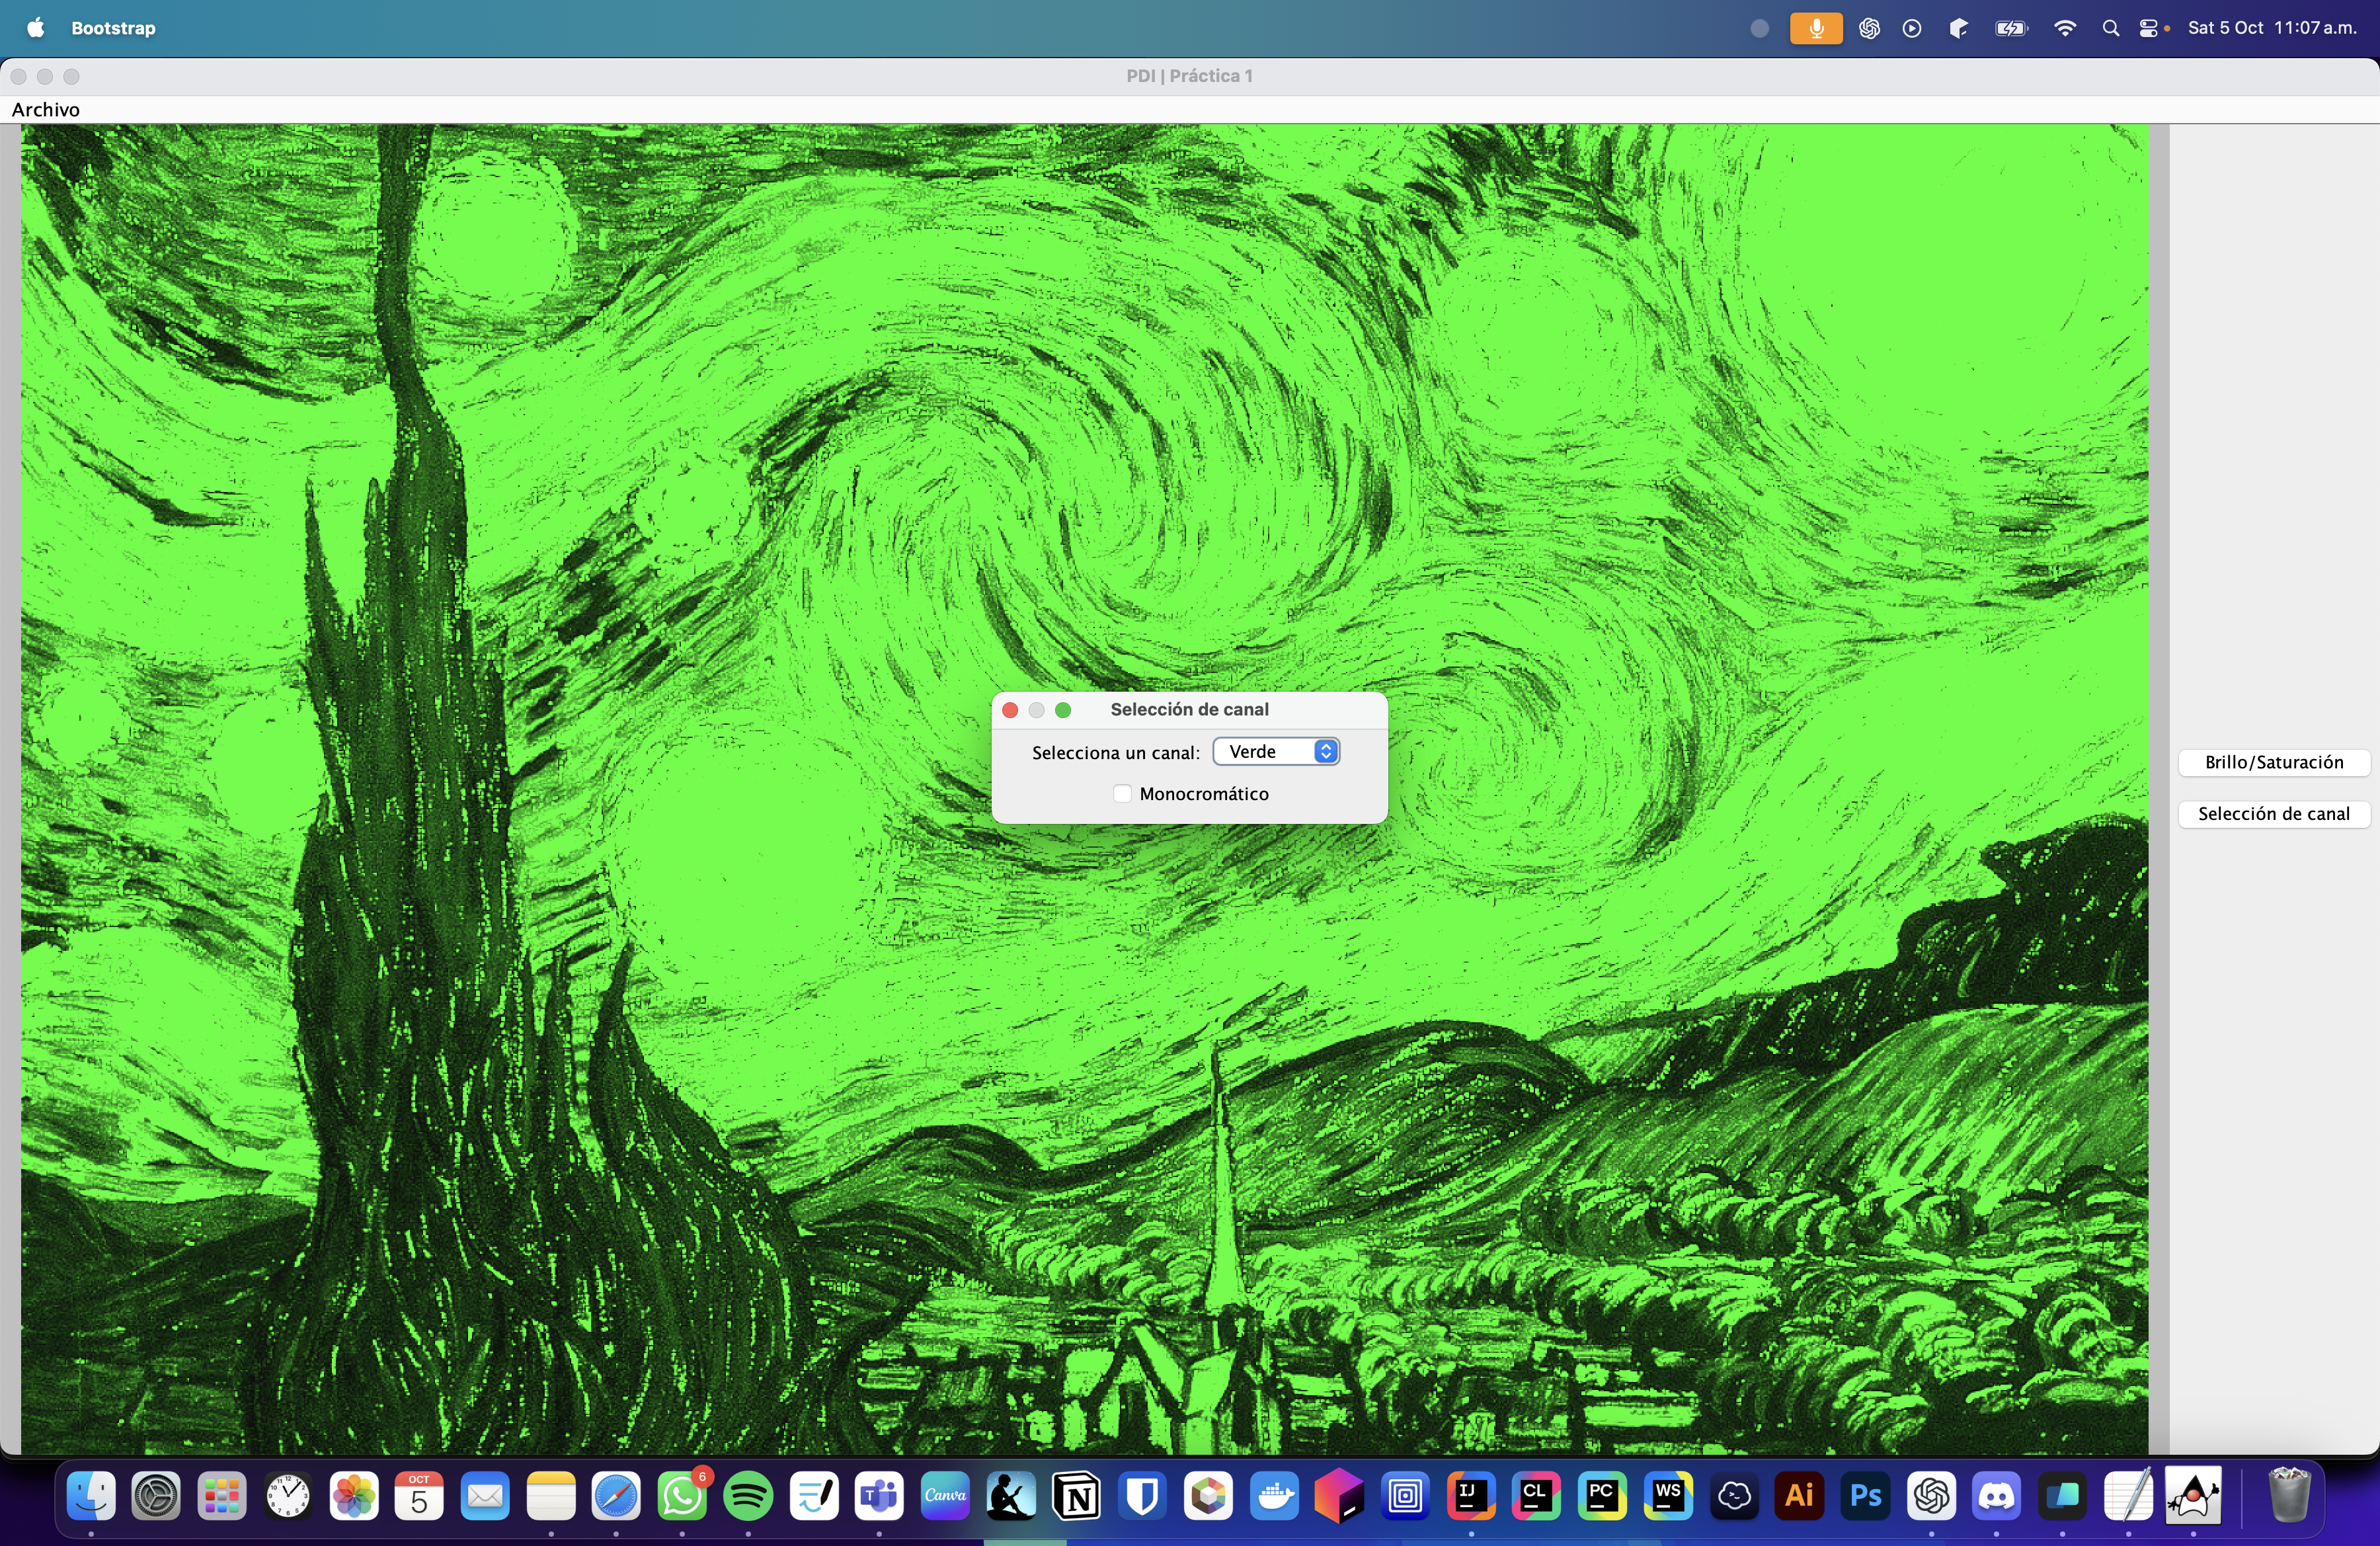
\includegraphics[width=\textwidth]{image/functionality/canal-verde}
    \caption{Visualización del canal verde}\label{fig:canal-verde}
  \end{figure}

  \subsection{Canal Azul}\label{subsec:canal-azul}
  \begin{figure}[H]
    \centering
    \includegraphics[width=\textwidth]{image/functionality/canal-azul}
    \caption{Visualización del canal azul}\label{fig:canal-azul}
  \end{figure}


  \section{Aplicación de Filtro Monocromático}\label{sec:aplicacion-de-filtro-monocromatico}
  El usuario también puede aplicar un filtro monocromático para convertir la imagen a escala de grises.

  \begin{figure}[H]
    \centering
    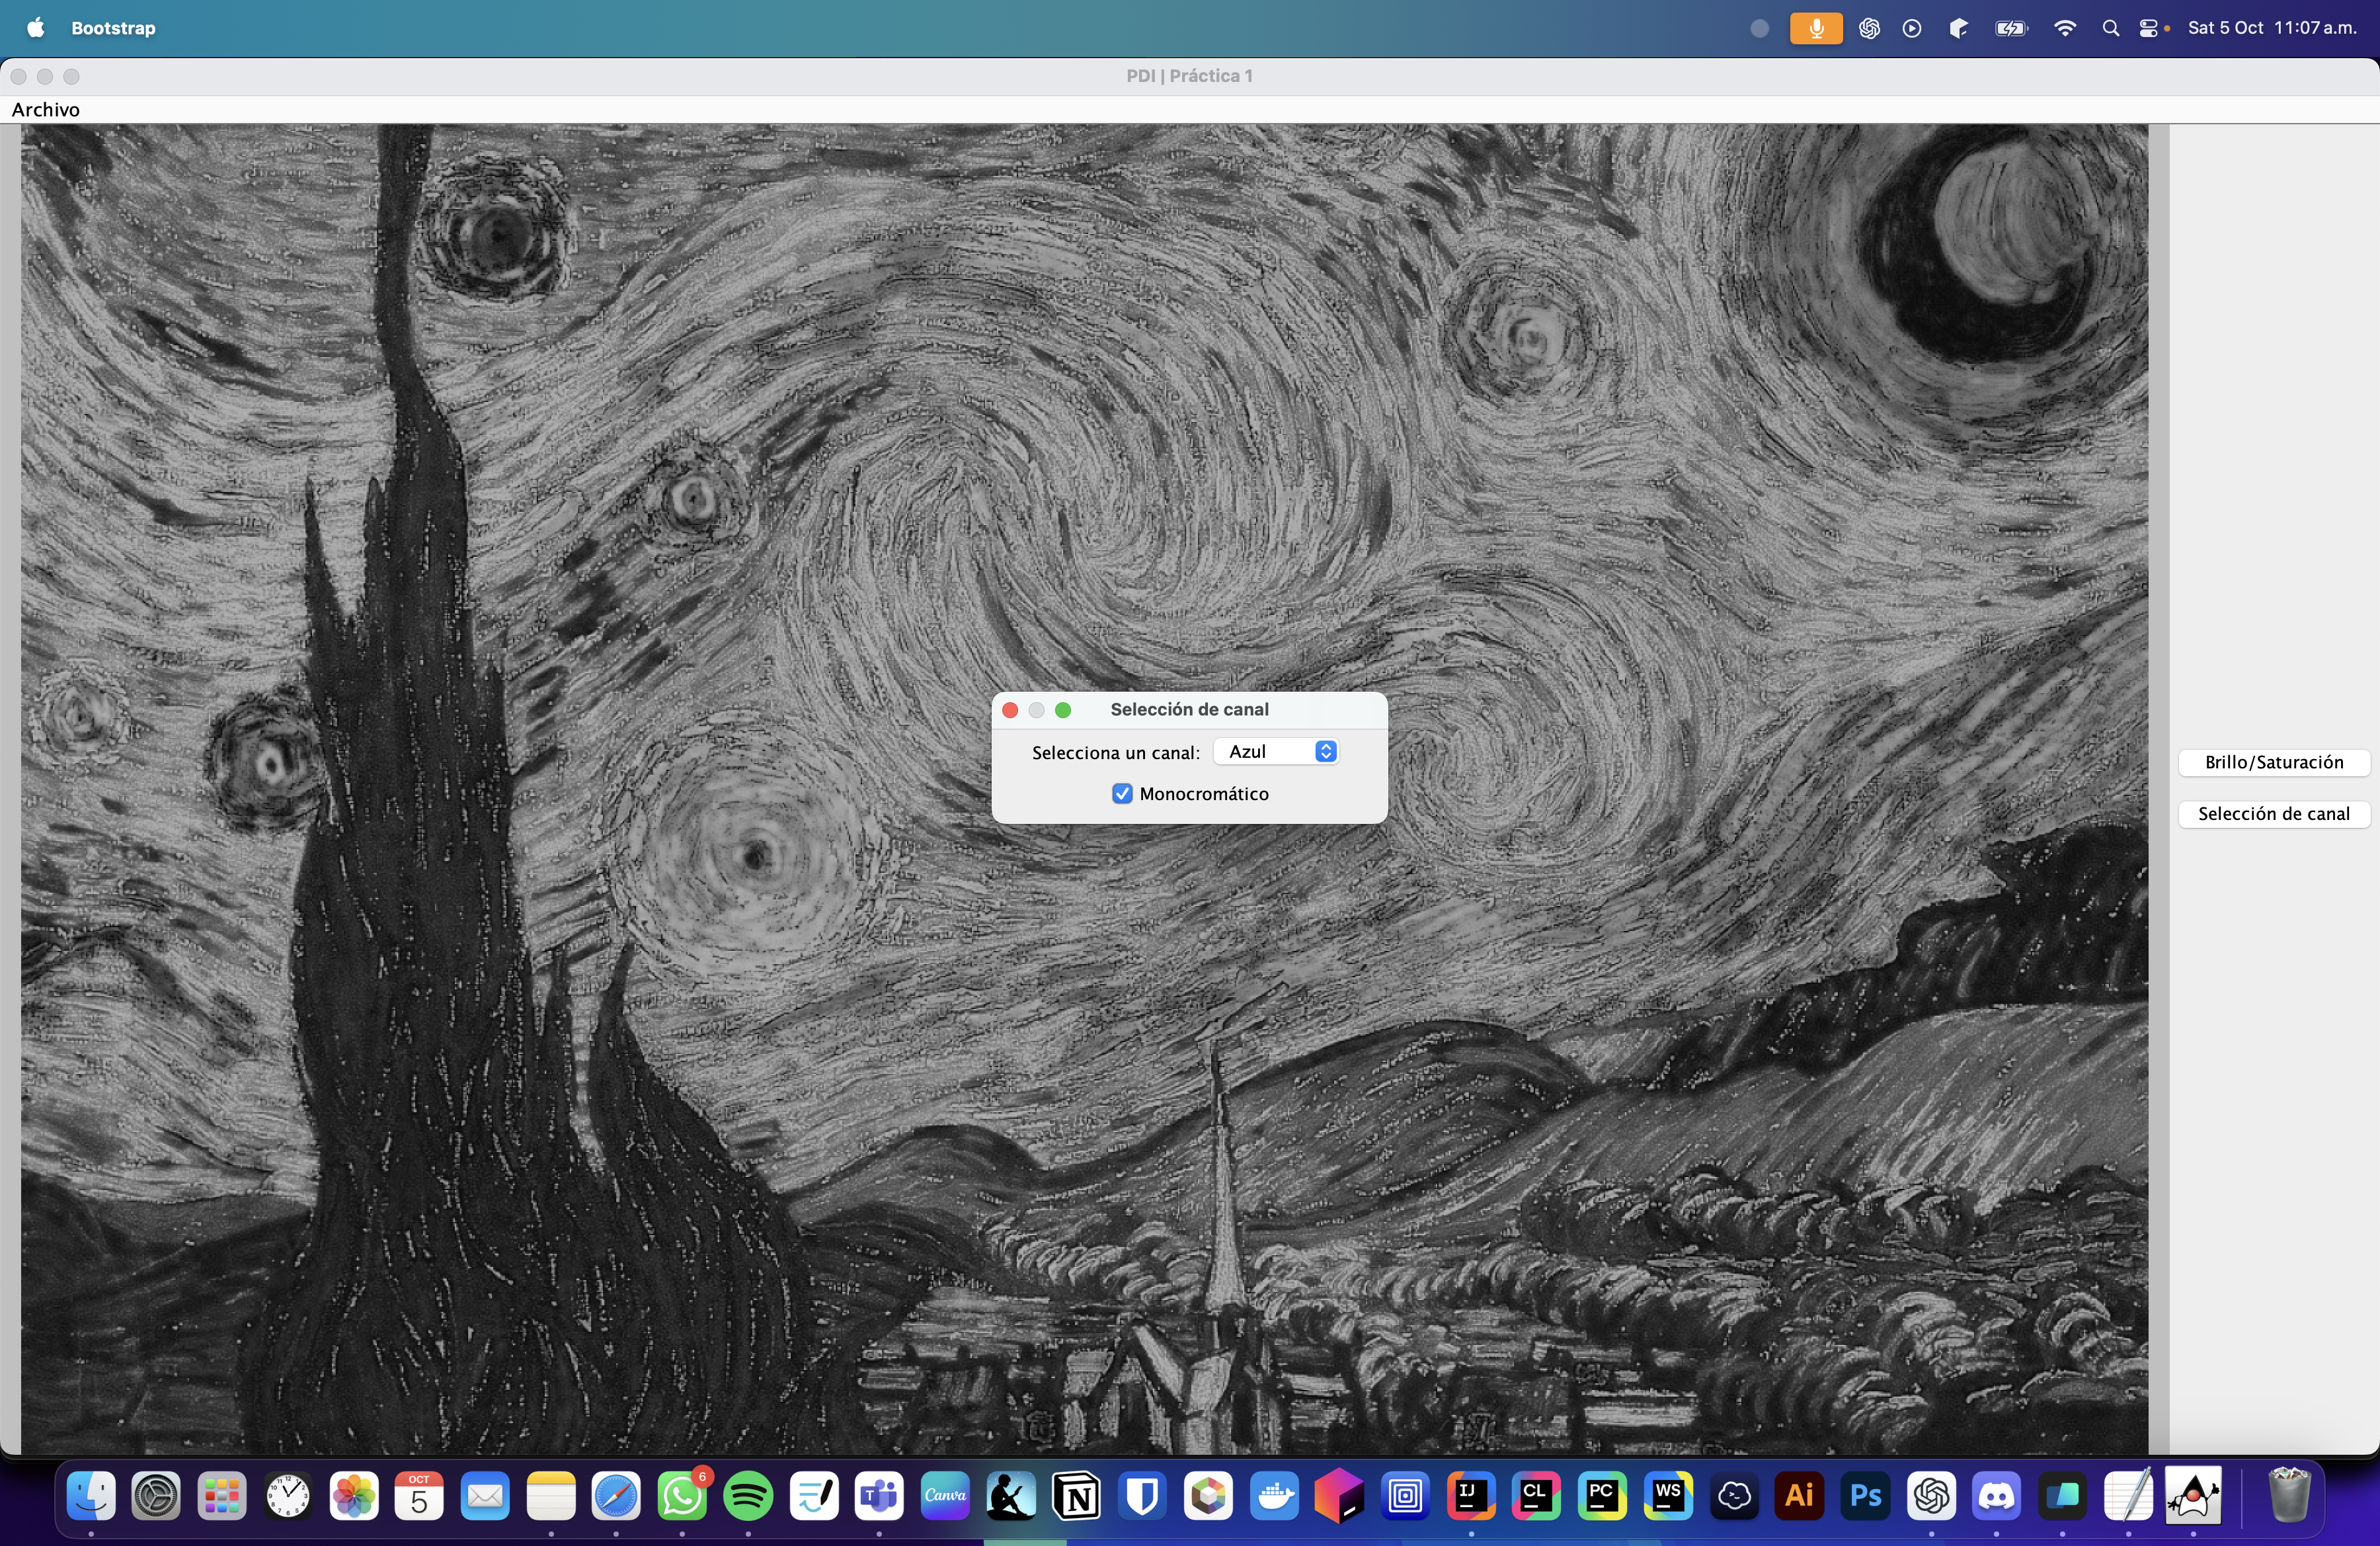
\includegraphics[width=\textwidth]{image/functionality/monocromatico}
    \caption{Aplicación del filtro monocromático}\label{fig:monocromatico}
  \end{figure}


  \section{Guardado de la Imagen Modificada}\label{sec:guardado-de-la-imagen-modificada}
  Una vez que la imagen ha sido modificada, el usuario puede guardarla, seleccionando el nombre y la ubicación en su sistema de archivos.

  \begin{figure}[H]
    \centering
    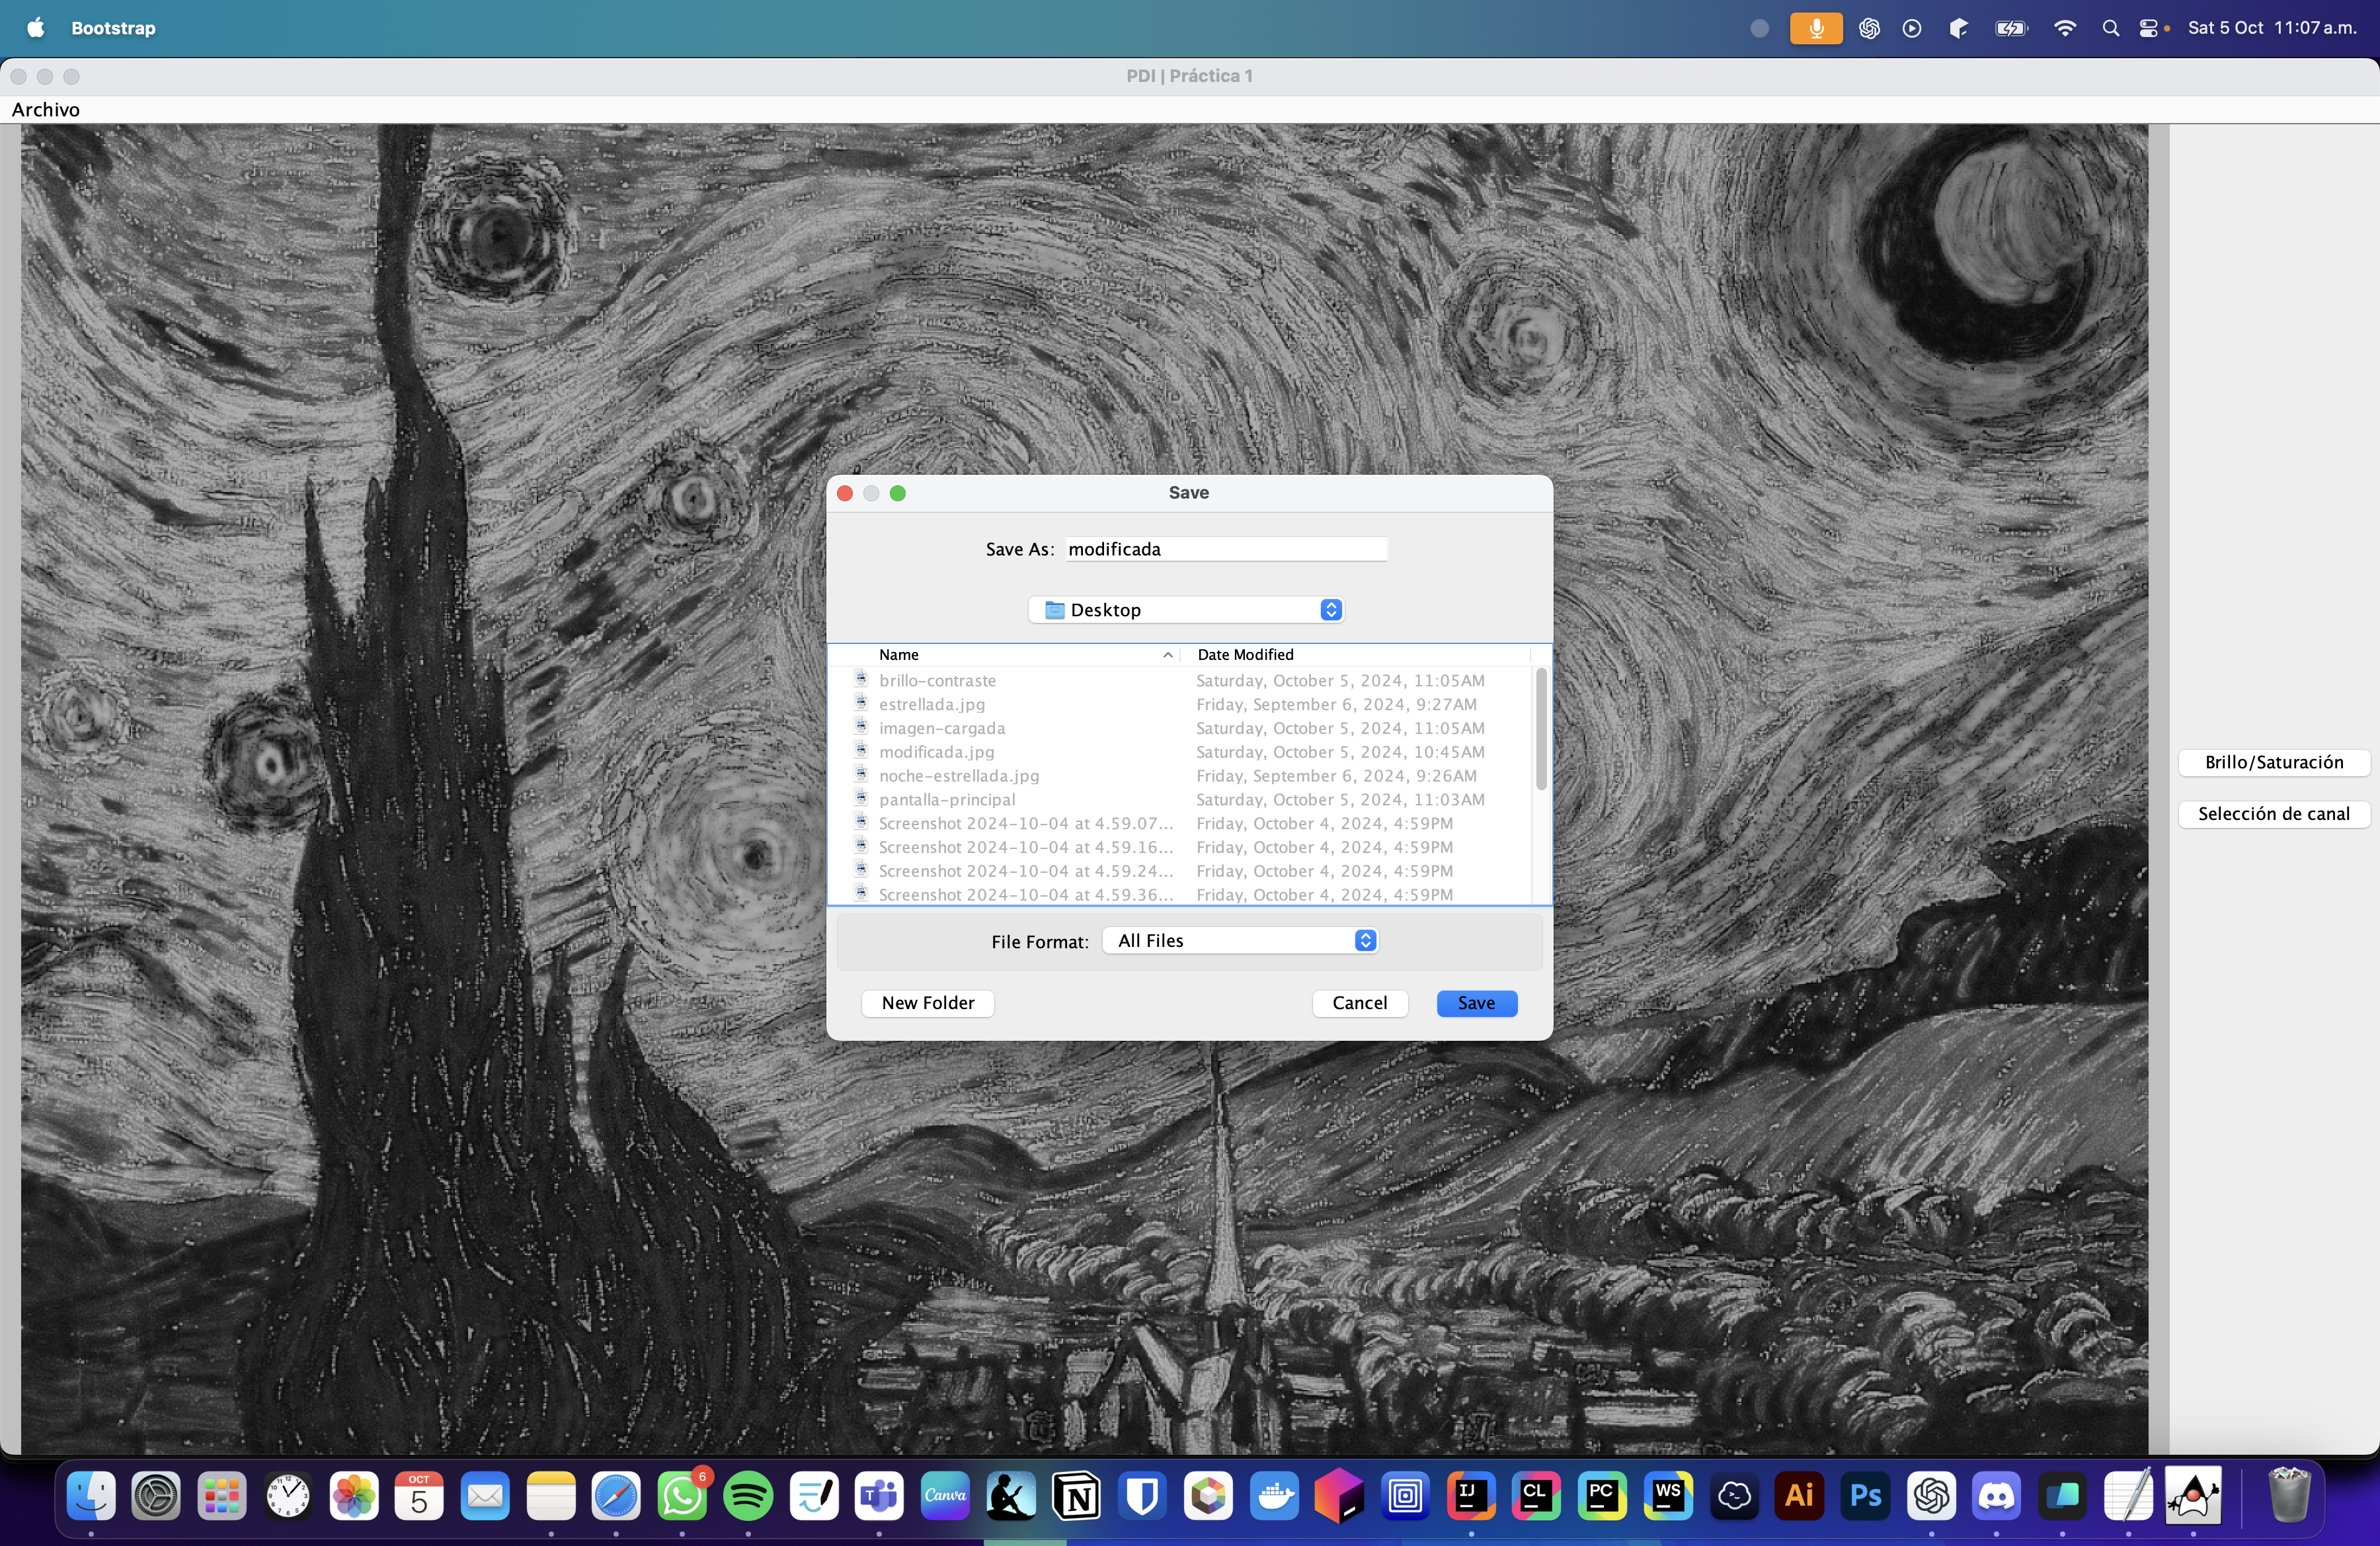
\includegraphics[width=\textwidth]{image/functionality/guardar}
    \caption{Guardado de la imagen modificada}\label{fig:guardar}
  \end{figure}


  \section{Visualización de la Imagen Guardada}\label{sec:visualizacion-de-la-imagen-guardada}
  Finalmente, la imagen guardada puede ser abierta y visualizada con el visor de imágenes del sistema operativo.

  \begin{figure}[H]
    \centering
    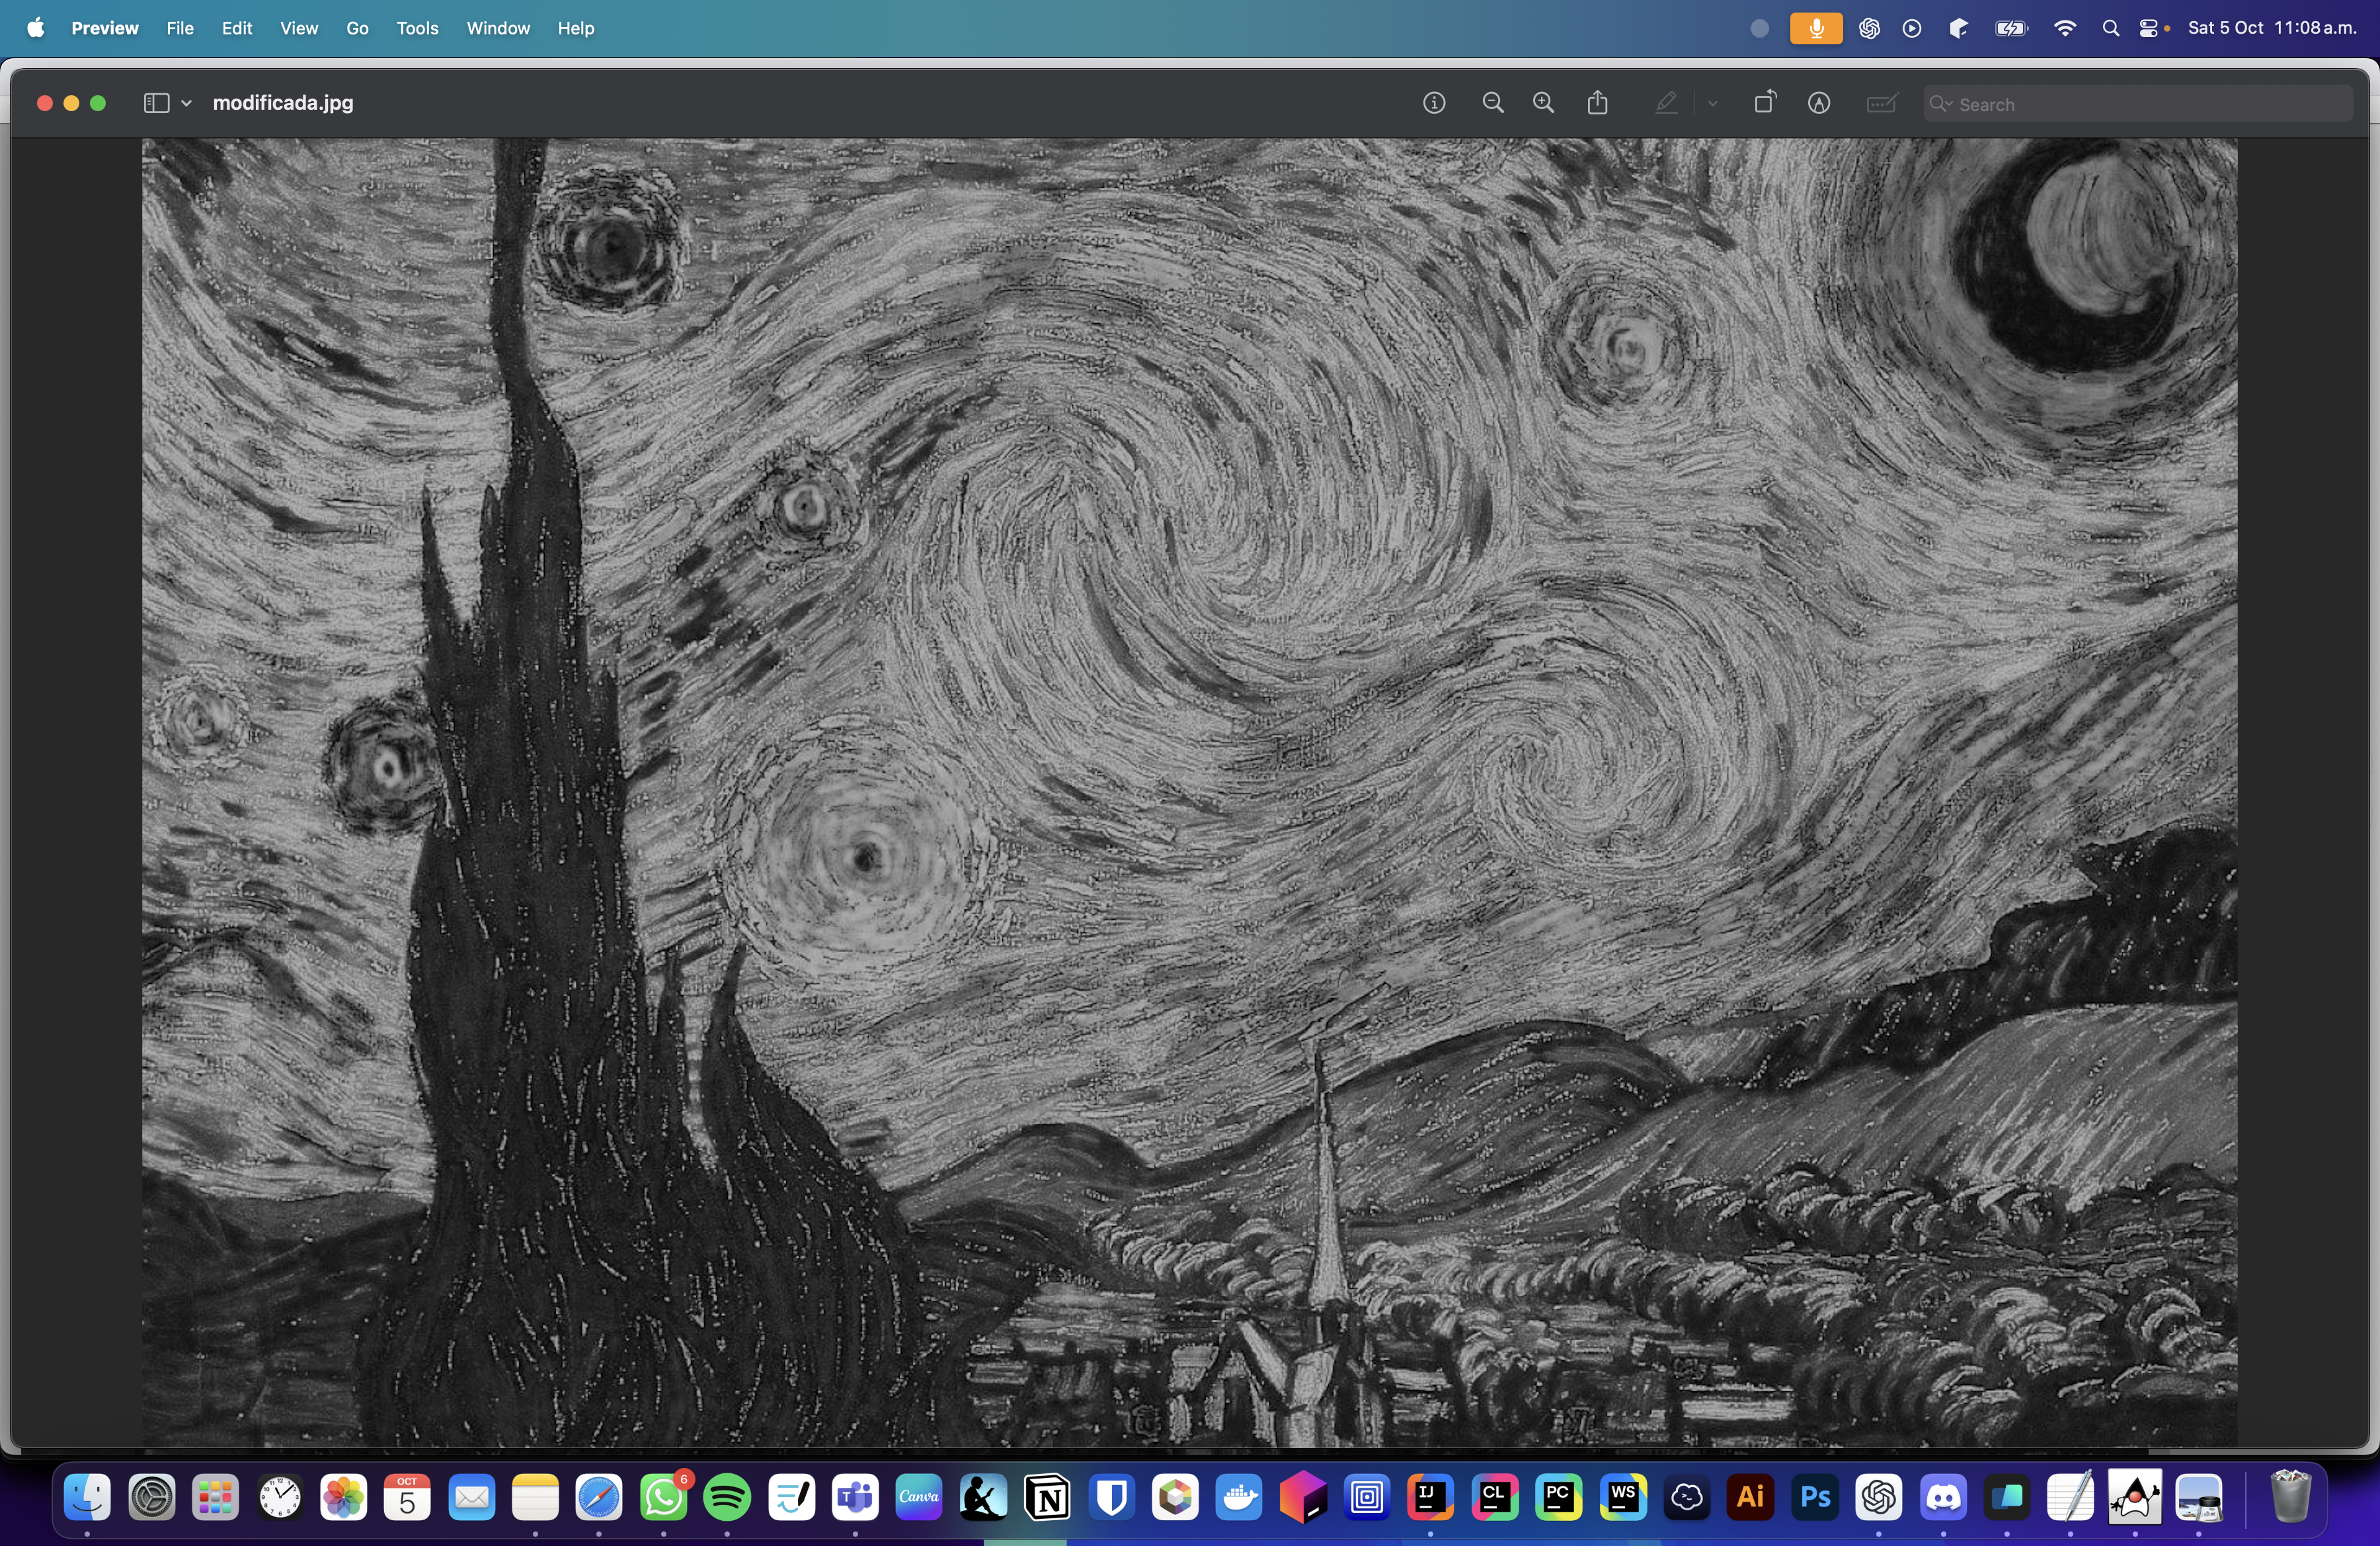
\includegraphics[width=\textwidth]{image/functionality/guardada}
    \caption{Imagen modificada guardada visualizada}\label{fig:guardada}
  \end{figure}


  \chapter{Conclusión}\label{ch:conclusion}
  Esta práctica fue fundamental para entender cómo las imágenes pueden ser manipuladas a nivel de píxel utilizando Java.
  Al trabajar con las APIs de Swing y AWT, se aprendió cómo construir interfaces gráficas interactivas, lo cual es clave en muchas aplicaciones modernas.

  Una de las principales conclusiones es la importancia de la modularidad en el diseño de software.
  Al dividir el código en clases específicas, fue posible mantener una estructura clara y fácil de mantener.
  Además, el uso de interfaces permitió la creación de nuevos procesadores de píxeles sin alterar el código existente, lo que demuestra la flexibilidad del diseño orientado a objetos.

  Como mejora, se podría extender la funcionalidad de la aplicación para soportar más formatos de imagen, o incluir algoritmos de procesamiento más avanzados, como la detección de bordes o la segmentación de imágenes.
  También se podría optimizar el rendimiento para manejar imágenes de mayor resolución sin comprometer la velocidad de procesamiento.

  Finalmente, esta práctica proporcionó una experiencia valiosa en la creación de aplicaciones gráficas y en el procesamiento de imágenes, temas que son esenciales en el campo de la visión por computadora y la inteligencia artificial.

\end{document}
